% \documentclass{article}
% % \usepackage[utf8]{inputenc}
% \usepackage{fullpage}
% \usepackage {setspace}
% \usepackage[hang,flushmargin]{footmisc} %control footnote indent
% \usepackage{url} % for website links
% \usepackage{amssymb,amsmath}%for matrix
% \usepackage{graphicx}%for figure
% \usepackage{appendix}%for appendix
% \usepackage{float}
% \usepackage{multirow}
% \usepackage{longtable}
% \usepackage{morefloats}%in case there are too many float tables and figures
% \usepackage{caption}
% \usepackage{subcaption}
% \usepackage{listings}
% \captionsetup[subtable]{font=normal}
% \usepackage{color}
% \usepackage{hyperref}
% \usepackage[round]{natbib}
% \usepackage[export]{adjustbox}
% %\usepackage{Sweave}
% \setlength{\parindent}{0em}
% \setlength{\parskip}{0.5em}


% \graphicspath{{0.plots/}}


% \begin{document}
\subsection{Application}\label{sec:p3application}
\subsubsection{The Atherosclerosis Risk in Communities (ARIC) Study}\label{sec:p3data}
%%%% briefly talk about which data will be used then talk about clinical background of HD
In this section, we apply the proposed joint models to the data from the Atherosclerosis Risk in Communities Study (ARIC). ARIC is a prospective epidemiological study conducted in four diverse U.S. communities (i.e. Forsyth County in North Carolina, Jackson County in Mississippi, Minneapolis suburbs in Minnesota, and Washington County in Maryland). The aims of ARIC study are to investigate the causes of atherosclerosis and its clinical outcomes, and variation in cardiovascular risk factors, medical care, and disease by race, gender, location, and date \citep{aric1989atherosclerosis}. There are two components in ARIC study, the cohort component and the community surveillance component. In the cohort component, a cohort sample of approximately 4000 individuals aged 45 $-$ 64 years were randomly selected from each of the four ARIC field centers as the representative of the community to receive extensive follow-up study. The data used in this work is from the cohort component.

One of the objectives of the cohort study is to investigate the trends in rates of hospitalized myocardial infarction (MI) and coronary heart diseases (CHD) in those communities. From previous studies it is known that risk factors for CHD differ significantly by race group. \cite{wattanakit2005risk, rodriguez2014systolic} also showed that systolic blood pressure (SBP) was an important risk factor for CHD events in the ARIC data. However, few studies have considered the time change rate of SBP among hypertensive patients, especially the time effect on different quantiles of SBP, and its association with the risk of recurrent CHD events. Thus, in this study, we aim to use longitudinal quantile regression to study the baseline covariate effects and time change rate on different quantiles of SBP and to characterize the association between SBP trajectory and recurrence of CHD events.

Data used in this work is derived from one of the four study communities (center ID is de-identified in the data), in which we include only white hypertensive participants (with SBP $>$ 140 mm Hg and DBP $>$ 90 mm Hg at baseline or self-reported history of physician-diagnosed hypertension or taking anti-hypertensive medicine). Participants who had prevalent CHD (defined by Q waves on the electrocardiogram, self-reported history of MI diagnosis, coronary artery bypass graft, or coronary angioplasty) before the first examination are excluded from the analysis. The resulting study cohort consists of 657 participants. Repeated measures of SBP were collected from the four longitudinal examination cycles that started at 1987 and ended at 1998 (i.e. 1987 $-$ 1989, 1990 $-$ 1992, 1993 $-$ 1995, and 1996 $-$ 1998). Out of the total 657 participants, 440 (67\%) individuals had four complete SBP measures, 113 (17\%), 54 (8\%), and 50 (8\%) had three, two and only one measure respectively. The LOESS curve in Figure ~\ref{fig:sbp_loess} shows no obvious time trend for SBP in approximately 11-year follow-up period. Follow-up for recurrent CHD events continued through 2010. The median follow-up time is 21 years with the maximum as 24 years. 242 (36\%) deaths occurred during the follow-up and 115, 31, and 17 patients experienced one, two or more than two CHD events. Summary of the baseline characteristics of the study cohort can be found in Appendices Table ~\ref{tab:p3cht_baseline}.


\begin{figure}[ht]
\centering
% 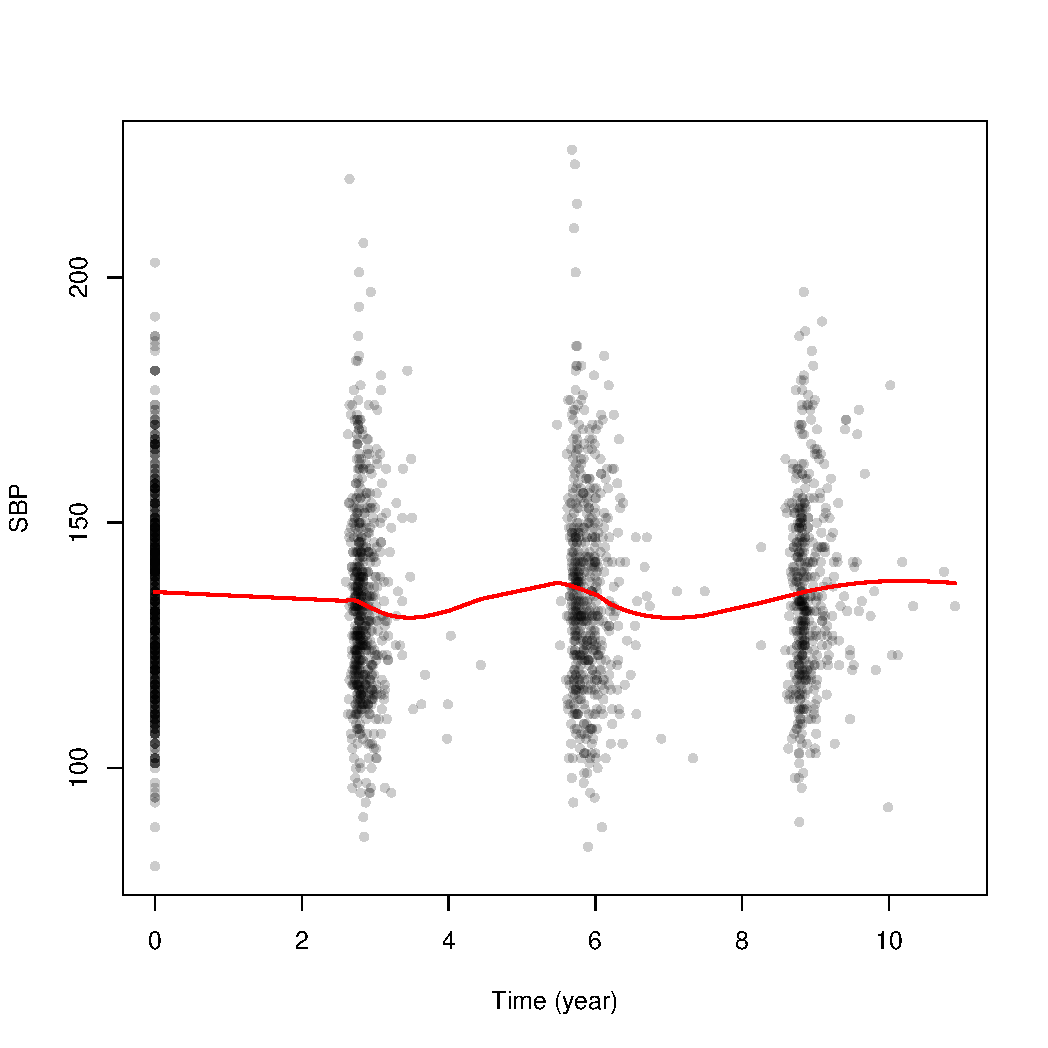
\includegraphics[width=\columnwidth]{SBP_loess.pdf}
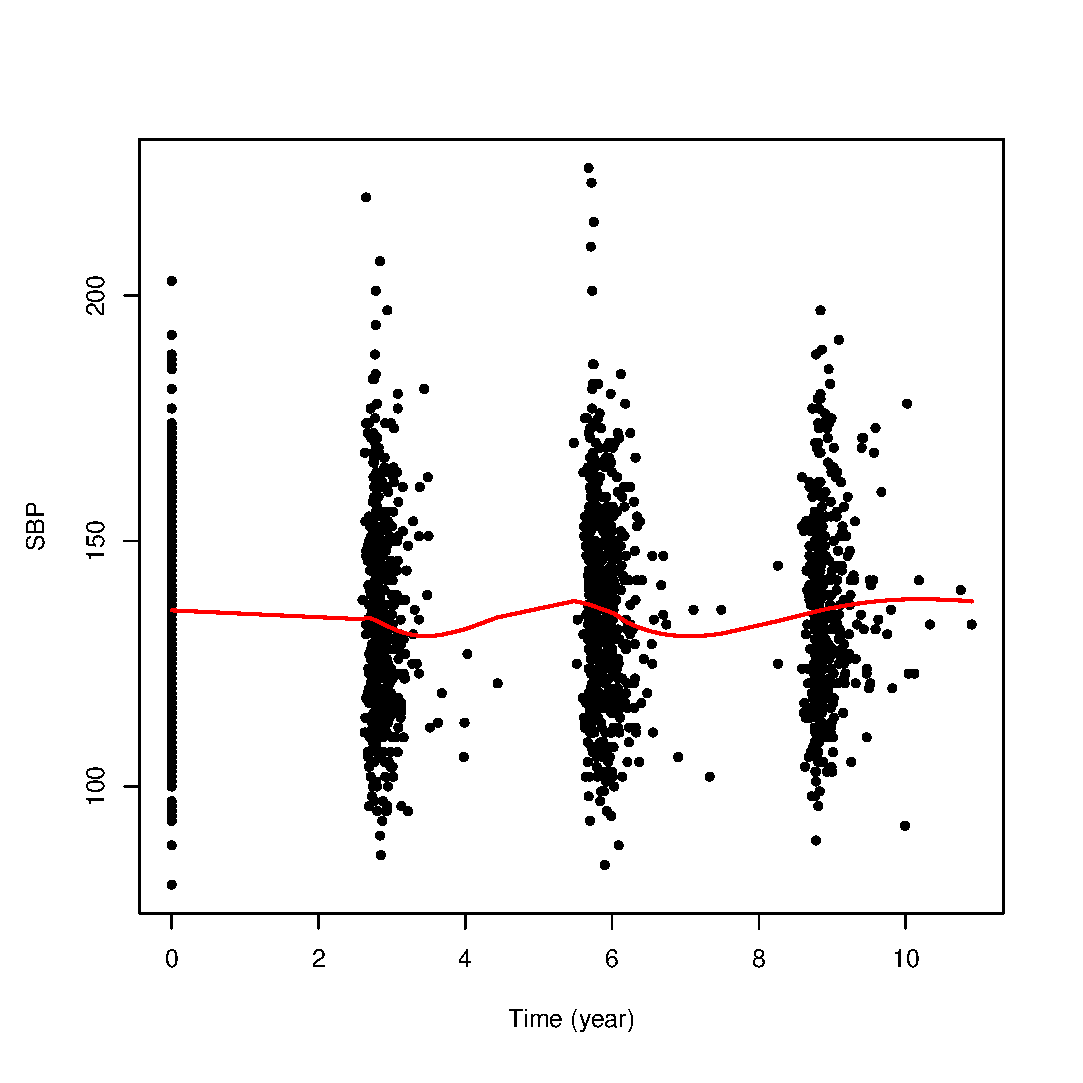
\includegraphics[scale=0.6]{SBP_loess.eps}
\caption{Scatter plot with LOESS curve of longitudinal SBP measures in the study cohort.}
\label{fig:sbp_loess}
\end{figure}

In data analysis, follow-up time is converted from days to years and the first examination date is set to time 0; baseline age is centered by subtracting the overall mean, and total-cholesterol is standardized to have mean 0 and standard deviation 1. We consider the following JM:
\small{
\begin{equation*}\label{eqn:p3data_joint}
\left\{
\begin{array}{l}
sbp_{i}(t) = m_{i}(t) + \varepsilon_{i}(t) = \beta_0 + \beta_1 age_{0i} + \beta_2 chol_i + \beta_3 I_{hyper-med_i}+ \beta_4 t + {u}_{i1} + u_{i2} t + \varepsilon_{i}(t)\\
r_i(t|\mathcal{M}_{i}(t);  \boldsymbol{\gamma}, \alpha) = r_{0}(t)v_i\exp(\gamma_1 I_{male_i} + \gamma_3 I_{smoke_i} + \gamma_4I_{diabetes_i} + \alpha m_i(t))
\end{array}
\right.
\end{equation*}
}
where we assume  $\varepsilon_{i}(t)\sim ALD(0, \sigma, \tau)$. $age_0$ is the baseline age at the first examination, $chol$ stands for the total-cholesterol level (mg/dL), $I_{hyper-med}$ is the variable indicating whether an individual had taken hypertension lowering medication, $t$ is the follow-up time, and $u_{i1}$ and $u_{i2}$ are subject-specific random intercept and slope to account for the within subject correlation and between subject variation. In the recurrent events submodel, we specify a piecewise constant baseline intensity function with three time intervals, where $\lambda_k$ is the hazard rate for time interval $[t_{k-1}, t_{k})$, that is $I_k(t)=1$ if $t\in[t_{k-1}, t_{k})$ and 0 otherwise. Knots $t_1$ and $t_2$, used to define piecewise constant time intervals, are selected as the 33.3\% and 66.7\% percentiles of the ordered follow-up time; while $t_0$ = 0 and $t_3$ is the maximum of follow-up time. We also include a frailty term $v_i$ in the recurrent events model that introduces correlation of multiple CHD events within the same individual. Other model covariates include indicator variables for male ($I_{male}$), ever smoke ($I_{smoke}$), and diabetes mellitus ($I_{diabetes}$). In above QRJM, the true underlying longitudinal measure of SBP is treated as a time dependent covariate in the recurrent event process and $\alpha$ is the association parameter governing the dependence between these two processes. Two chains with diverse initial values are initiated in the Bayesian inference algorithm and the chains are considered to converge if the potential scale reduction factors (PSRF) for all parameters are below 1.1.

We select 80\% of the study cohort (i.e. 526 subjects) to draw parameter inference, based on which we then make predictions of CHD event probability for the rest 131 individuals. Inference results and interpretation can be found in Appendices Table~\ref{p3realdata_inference} and will not be discussed further here. In stead, we focus on presenting the predictions result in the following subsection.


\subsubsection{Dynamic Predictions of Recurrent CHD Event Risk}\label{sec:p3data_results}
To demonstrate how the model works in making subject-specific dynamic predictions of recurrent CHD event risk (in terms of event-free probability), we select three subjects (4, 55, and 65) with distinct data features as the representatives. Figure~\ref{plot:p3realdata_pred_surv_qt50} has three panels with increasing follow-up time in years. For each follow-up time $t$, we make predictions of CHD event-free probability for 1, 2, and 3 years in the future. There are some interesting findings that we would like to highlight: (i) patients who had more CHD events are predicted to have higher risk of CHD recurrence in the future. For example, subject 55 had three CHD events (the most among the three subjects) before year 9 and his/her predicted event-free probability is the lowest (or the highest risk) among the three, followed by subject 65, who had only one event. And subject 4, who didn't have any event occur at year 9, is predicted to only have small probabilities of CHD event in the near future. (ii) With longer follow-up time but no additional event, the predicted event-free probability improves. For example, in subject 55, there is no additional event occurs from $t=12$ to $t=14$ and the predicted event-free probabilities based on $t=14$ are higher than those from $t=12$ for the same $t+\Delta t$ values. (iii) Wider credible interval for larger prediction time window. This makes sense as the prediction uncertainty is higher for further time in the future.

Furthermore, we make the predictions for the whole testing data with three conditional quantiles (0.25, 0.50, and 0.75) of SBP. We summarize the predictive accuracy and present it in Table~\ref{tab:p3data_auc} using AUC, AARD and MRD. First, for the same follow-up time $t$, predictive accuracy is best with smallest $\Delta t$ and decreases when $\Delta t$ increases. This is probably because in this data set majority of the patients didn't have any event observed during the study follow-up and the predicted event-free probability didn't decrease significantly with larger $\Delta t$, thus it is more difficult for the model to differentiate those who will versus who will not have CHD event in the longer future since the predictions are close to each other. Second, with longer follow-up time, the predictive accuracy improves accordingly. This finding is consistent with what we observed in the simulation study and it probably dues to the effect of additional longitudinal and recurrent events information used in making predictions. In additional, we also calculate the AUC for the predictions made from the traditional LMJM model. Compared with LMJM, QRJM has better predictive accuracy at some quantiles, but not all. This is because some conditional quantiles of the SBP can be more informative in predicting future recurrent events than the conditional mean while some are not.


\begin{figure}[H]
\captionsetup[subfloat]{farskip=-5pt,captionskip=-1pt}
\centering
\subfloat[Predictions based on follow-up time $t = $ 9]{
    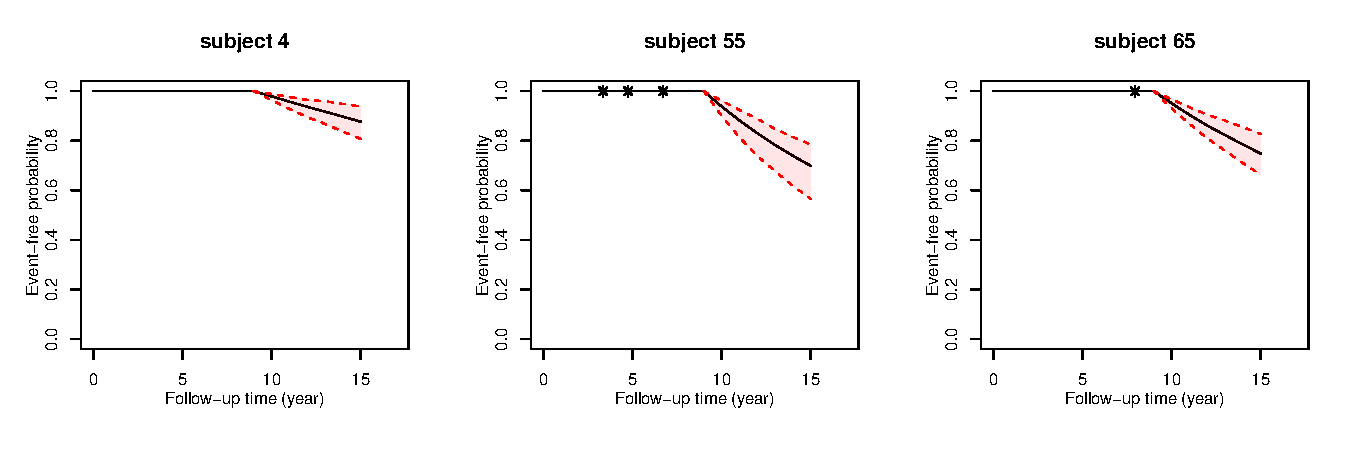
\includegraphics[width=\columnwidth]{qt50_80pct_t9_dt123456.pdf}\label{plot:p3realdata_pred_surv_t9}
}

\centering
\subfloat[Predictions based on follow-up time $t=$ 12]{
    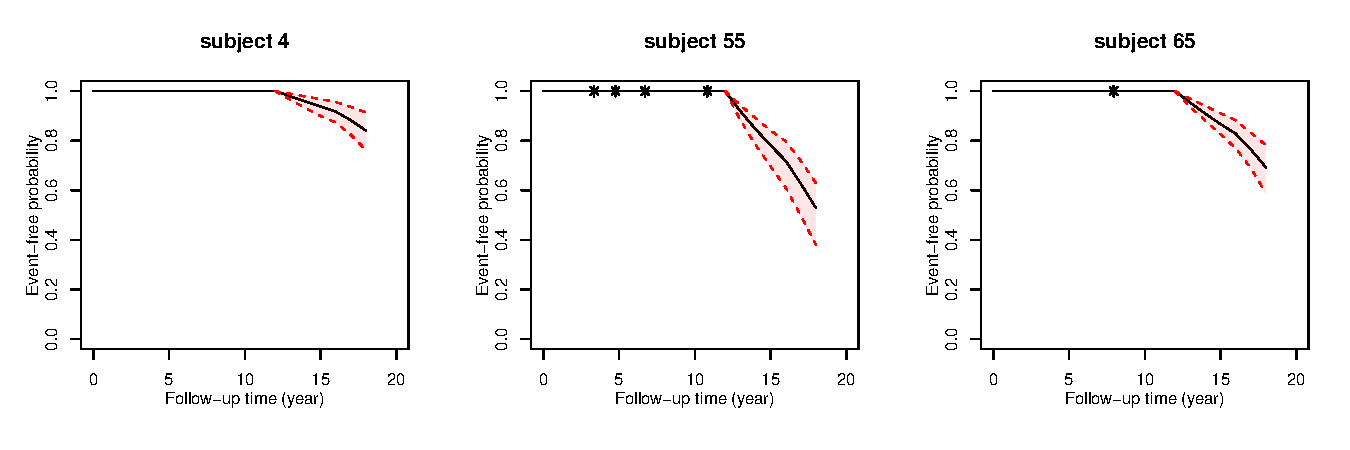
\includegraphics[width=\columnwidth]{qt50_80pct_t12_dt123456.pdf}\label{plot:p3realdata_pred_surv_t16}
}

\centering
\subfloat[Predictions based on follow-up time $t=$ 14]{
    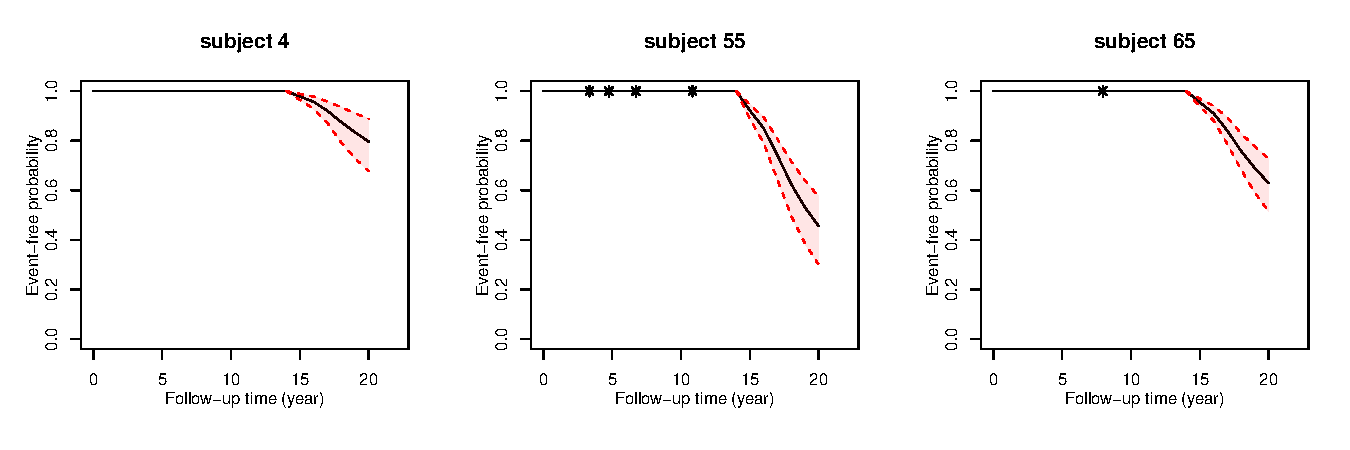
\includegraphics[width=\columnwidth]{qt50_80pct_t14_dt123456.pdf}\label{plot:p3realdata_pred_surv_t18}
}
  \caption{ARIC data analysis: Dynamic predictions of CHD event-free probability, based on various follow-up time and prediction time window, with 95\% credible interval from QRJM at $\tau=0.5$ for selected subjects ($*$ indicates CHD event).}
  \label{plot:p3realdata_pred_surv_qt50}
\end{figure}





\begin{table}[H]
\centering
\caption{ARIC data analysis: AUC, AARD and MRD of the predictions of CHD event-free probability from QRJM and AUC from LMJM.}
\label{tab:p3data_auc}
\adjustbox{max width=\textwidth}{
\begin{tabular}{rrrrrrrrrrrrrrc}
\hline
$t$ & $\Delta t$ & \multicolumn{3}{c}{AUC ($\tau$)} & & \multicolumn{3}{c}{AARD ($\tau$)} & & \multicolumn{3}{c}{MRD ($\tau$)} & & \multirow{2}{*}{AUC (LMJM)}\\
\cline{3-5}  \cline{7-9} \cline{11-13}
\multicolumn{2}{c}{(year)}  & 0.25 & 0.50 & 0.75 & & 0.25 & 0.50 & 0.75 & & 0.25 & 0.50 & 0.75 & & \\
\hline
\multirow{3}{*}{$9$}  & 1 & 0.726 & 0.713 & 0.712 && 0.357 & 0.327 & 0.327 &&  0.035 & 0.032 & 0.034 & &0.717\\
            & 2 &  0.685 & 0.671 & 0.670 &&  0.286 & 0.255 & 0.255 && 0.028 & 0.024 & 0.025 && 0.676\\
            & 3 &  0.669 & 0.654 & 0.654 &&  0.257 & 0.227 & 0.228 && 0.027 & 0.022 & 0.023  & &0.659\\[0.5em]
\multirow{3}{*}{$12$}  & 1 & 0.770 & 0.756 & 0.754  && 0.434 & 0.402 & 0.400 &&  0.056 & 0.053 & 0.053 & &0.761\\
            & 2 &  0.721 & 0.703 & 0.703 && 0.345 & 0.303 & 0.304 && 0.044 & 0.039 & 0.039 & &0.710\\
            & 3 & 0.699 & 0.680 & 0.680 &&  0.307 & 0.266 & 0.267 && 0.042 & 0.035 & 0.035 & &0.687\\[0.5em]
\multirow{3}{*}{$14$}  & 1 &  0.797 & 0.784 & 0.784 &&  0.487 & 0.463 & 0.464 && 0.071 & 0.068 & 0.069 & &0.789\\
            & 2 & 0.748 & 0.731 & 0.732  && 0.394 & 0.355 & 0.357  &&  0.059 & 0.054 & 0.054 & &0.738\\
            & 3 &  0.714 & 0.695 & 0.697 && 0.331 & 0.288 & 0.293  && 0.059 & 0.049 & 0.050 & &0.704\\
\hline
\end{tabular}
}
\end{table}










% \end{document}
